\documentclass{article}
\usepackage[margin=0.75in]{geometry}
\usepackage[utf8]{inputenc}
\usepackage[section]{placeins}
\usepackage{graphicx}
\graphicspath{{./images/}}
\usepackage{float}
\usepackage{listings}
\usepackage{framed}


\begin{document}

These are old and possibly not going to be looked at again, altough
it's very possible that they will be so I'm keeping them here in
its own document

\section{Dacapo Tests}
Running the benchmark while measuring
\begin{itemize}
\item num reads between consecutive nonzero readings
\item nonzero energy reading values
\item time between nonzero readings
\end{itemize}

Interesting that GPU has no results with some benchmarks and more results with some benchmarks. GPU's RAPL counter
value usually stays at the same level (no increase) when I do my normal jRAPL running on this computer with no
benchmarks. But only some times. I honestly don't know what's going on with that, to be honest. Lately
I've been seeing more actual increases in GPU energy activity. I don't know if since I started using some of
the Dacapo benchmarks it "unlocked" GPU activity in my computer by actively stressing the systems that needed it,
but I'm honestly not sure. Something to keep in mind and keep an eye on, I suppose.

\subsection{avrova}
    
    \begin{figure}[H]
    	\centering
    	\includegraphics[width=17cm,height=20cm,keepaspectratio]{Dacapo_SystemC/avrova/PKG-scatter.png}
    	\caption{pkg dacapo avrova}
    	\label{fig:avrova-PKG}
    \end{figure}

    \begin{figure}[H]
    	\centering
    	\includegraphics[width=17cm,height=20cm,keepaspectratio]{Dacapo_SystemC/avrova/CORE-scatter.png}
    	\caption{core dacapo avrova}
    	\label{fig:avrova-CORE}
    \end{figure}
    \begin{figure}[H]
    	\centering
    	\includegraphics[width=17cm,height=20cm,keepaspectratio]{Dacapo_SystemC/avrova/DRAM-scatter.png}
    	\caption{dram dacapo avrova}
    	\label{fig:avrova-DRAM}
    \end{figure}
    \begin{figure}[H]
    	\centering
    	\includegraphics[width=17cm,height=20cm,keepaspectratio]{Dacapo_SystemC/avrova/GPU-scatter.png}
    	\caption{gpu dacapo avrova}
    	\label{fig:avrova-GPU}
    \end{figure}
  ]
\subsection{fop}
    \begin{figure}[H]
    	\centering
    	\includegraphics[width=17cm,height=20cm,keepaspectratio]{Dacapo_SystemC/fop/CORE-scatter.png}
    	\caption{core dacapo results fop}
    	\label{fig:fop-CORE}
    \end{figure}
    \begin{figure}[H]
    	\centering
    	\includegraphics[width=17cm,height=20cm,keepaspectratio]{Dacapo_SystemC/fop/DRAM-scatter.png}
    	\caption{dram dacapo results fop}
    	\label{fig:fop-DRAM}
    \end{figure}
    \begin{figure}[H]
    	\centering
    	\includegraphics[width=17cm,height=20cm,keepaspectratio]{Dacapo_SystemC/fop/GPU-scatter.png}
    	\caption{gpu dacapo results fop}
    	\label{fig:fop-GPU}
    \end{figure}
    \begin{figure}[H]
    	\centering
    	\includegraphics[width=17cm,height=20cm,keepaspectratio]{Dacapo_SystemC/fop/PKG-scatter.png}
    	\caption{pkg dacapo results fop}
    	\label{fig:fop-PKG}
    \end{figure}

\subsection{h2}
    \begin{figure}[H]
    	\centering
    	\includegraphics[width=17cm,height=20cm,keepaspectratio]{Dacapo_SystemC/h2/CORE-scatter.png}
    	\caption{core dacapo results h2}
    	\label{fig:h2-CORE}
    \end{figure}
    \begin{figure}[H]
    	\centering
    	\includegraphics[width=17cm,height=20cm,keepaspectratio]{Dacapo_SystemC/h2/DRAM-scatter.png}
    	\caption{dram dacapo results h2}
    	\label{fig:h2-DRAM}
    \end{figure}
    \begin{figure}[H]
    	\centering
    	\includegraphics[width=17cm,height=20cm,keepaspectratio]{Dacapo_SystemC/h2/GPU-scatter.png}
    	\caption{GPU dacapo results h2}
    	\label{fig:h2-GPU}
    \end{figure}
    \begin{figure}[H]
    	\centering
    	\includegraphics[width=17cm,height=20cm,keepaspectratio]{Dacapo_SystemC/h2/PKG-scatter.png}
    	\caption{PKG dacapo results h2}
    	\label{fig:h2-PKG}
    \end{figure}
    

\subsection{jython}
    \begin{figure}[H]
    	\centering
    	\includegraphics[width=17cm,height=20cm,keepaspectratio]{Dacapo_SystemC/jython/CORE-scatter.png}
    	\caption{CORE dacapo results jython}
    	\label{fig:jython-CORE}
    \end{figure}
        \begin{figure}[H]
    	\centering
    	\includegraphics[width=17cm,height=20cm,keepaspectratio]{Dacapo_SystemC/jython/DRAM-scatter.png}
    	\caption{DRAM dacapo results jython}
    	\label{fig:fop-jython}
    \end{figure}
    \begin{figure}[H]
    	\centering
    	\includegraphics[width=17cm,height=20cm,keepaspectratio]{Dacapo_SystemC/jython/GPU-scatter.png}
    	\caption{GPU dacapo results jython}
    	\label{fig:jython-GPU}
    \end{figure}
    \begin{figure}[H]
    	\centering
    	\includegraphics[width=17cm,height=20cm,keepaspectratio]{Dacapo_SystemC/jython/PKG-scatter.png}
    	\caption{PKG dacapo results jython}
    	\label{fig:jython-PKG}
    \end{figure}

\subsection{luindex}
    \begin{figure}[H]
    	\centering
    	\includegraphics[width=17cm,height=20cm,keepaspectratio]{Dacapo_SystemC/luindex/CORE-scatter.png}
    	\caption{CORE dacapo results luindex}
    	\label{fig:luindex-CORE}
    \end{figure}
        \begin{figure}[H]
    	\centering
    	\includegraphics[width=17cm,height=20cm,keepaspectratio]{Dacapo_SystemC/luindex/DRAM-scatter.png}
    	\caption{DRAM dacapo results luindex}
    	\label{fig:luindex-DRAM}
    \end{figure}
    \begin{figure}[H]
    	\centering
    	\includegraphics[width=17cm,height=20cm,keepaspectratio]{Dacapo_SystemC/luindex/GPU-scatter.png}
    	\caption{GPU dacapo results luindex}
    	\label{fig:fop-GPU}
    \end{figure}
    \begin{figure}[H]
    	\centering
    	\includegraphics[width=17cm,height=20cm,keepaspectratio]{Dacapo_SystemC/luindex/PKG-scatter.png}
    	\caption{PKG dacapo results luindex}
    	\label{fig:luindex-PKG}
    \end{figure}

\subsection{lusearch}
    \begin{figure}[H]
    	\centering
    	\includegraphics[width=17cm,height=20cm,keepaspectratio]{Dacapo_SystemC/lusearch/CORE-scatter.png}
    	\caption{CORE dacapo results lusearch}
    	\label{fig:lusearch-CORE}
    \end{figure}
    \begin{figure}[H]
    	\centering
    	\includegraphics[width=17cm,height=20cm,keepaspectratio]{Dacapo_SystemC/fop/DRAM-scatter.png}
    	\caption{DRAM dacapo results lusearch}
    	\label{fig:fop-DRAM}
    \end{figure}
    \begin{figure}[H]
    	\centering
    	\includegraphics[width=17cm,height=20cm,keepaspectratio]{Dacapo_SystemC/lusearch/GPU-scatter.png}
    	\caption{GPU dacapo results lusearch}
    	\label{fig:lusearch-GPU}
    \end{figure}
    \begin{figure}[H]
    	\centering
    	\includegraphics[width=17cm,height=20cm,keepaspectratio]{Dacapo_SystemC/lusearch/PKG-scatter.png}
    	\caption{PKG dacapo results lusearch}
    	\label{fig:lusearch-PKG}
    \end{figure}
    
\subsection{lusearch-fix}
    \begin{figure}[H]
    	\centering
    	\includegraphics[width=17cm,height=20cm,keepaspectratio]{Dacapo_SystemC/lusearch-fix/CORE-scatter.png}
    	\caption{CORE dacapo results lusearch-fix}
    	\label{fig:lusearch-fix-CORE}
    \end{figure}
    \begin{figure}[H]
    	\centering
    	\includegraphics[width=17cm,height=20cm,keepaspectratio]{Dacapo_SystemC/lusearch-fix/DRAM-scatter.png}
    	\caption{DRAM dacapo results lusearch-fix}
    	\label{fig:lusearch-fix-DRAM}
    \end{figure}
    \begin{figure}[H]
    	\centering
    	\includegraphics[width=17cm,height=20cm,keepaspectratio]{Dacapo_SystemC/lusearch-fix/GPU-scatter.png}
    	\caption{GPU dacapo results lusearch-fix}
    	\label{fig:lusearch-fix-GPU}
    \end{figure}
    \begin{figure}[H]
    	\centering
    	\includegraphics[width=17cm,height=20cm,keepaspectratio]{Dacapo_SystemC/lusearch-fix/PKG-scatter.png}
    	\caption{PKG dacapo results lusearch-fix}
    	\label{fig:lusearch-fix-PKG}
    \end{figure}

\subsection{pmd}
    \begin{figure}[H]
    	\centering
    	\includegraphics[width=17cm,height=20cm,keepaspectratio]{Dacapo_SystemC/pmd/CORE-scatter.png}
    	\caption{CORE dacapo results pmd}
    	\label{fig:pmd-CORE}
    \end{figure}
    \begin{figure}[H]
    	\centering
    	\includegraphics[width=17cm,height=20cm,keepaspectratio]{Dacapo_SystemC/pmd/DRAM-scatter.png}
    	\caption{DRAM dacapo results pmd}
    	\label{fig:pmd-fix-DRAM}
    \end{figure}
    \begin{figure}[H]
    	\centering
    	\includegraphics[width=17cm,height=20cm,keepaspectratio]{Dacapo_SystemC/pmd/GPU-scatter.png}
    	\caption{GPU dacapo results pmd}
    	\label{fig:pmd-fix-GPU}
    \end{figure}
    \begin{figure}[H]
    	\centering
    	\includegraphics[width=17cm,height=20cm,keepaspectratio]{Dacapo_SystemC/pmd/PKG-scatter.png}
    	\caption{PKG dacapo results pmd}
    	\label{fig:pmd-fix-PKG}
    \end{figure}
    
\subsection{sunflow}
    \begin{figure}[H]
    	\centering
    	\includegraphics[width=17cm,height=20cm,keepaspectratio]{Dacapo_SystemC/sunflow/CORE-scatter.png}
    	\caption{CORE dacapo results sunflow}
    	\label{fig:sunflow-CORE}
    \end{figure}
    \begin{figure}[H]
    	\centering
    	\includegraphics[width=17cm,height=20cm,keepaspectratio]{Dacapo_SystemC/sunflow/DRAM-scatter.png}
    	\caption{DRAM dacapo results sunflow}
    	\label{fig:sunflow-fix-DRAM}
    \end{figure}
    \begin{figure}[H]
    	\centering
    	\includegraphics[width=17cm,height=20cm,keepaspectratio]{Dacapo_SystemC/sunflow/GPU-scatter.png}
    	\caption{GPU dacapo results sunflow}
    	\label{fig:sunflow-fix-GPU}
    \end{figure}
    \begin{figure}[H]
    	\centering
    	\includegraphics[width=17cm,height=20cm,keepaspectratio]{Dacapo_SystemC/sunflow/PKG-scatter.png}
    	\caption{PKG dacapo results sunflow}
    	\label{fig:sunflow-fix-PKG}
    \end{figure}
    


\subsection{tradebeans}
    \begin{figure}[H]
    	\centering
    	\includegraphics[width=17cm,height=20cm,keepaspectratio]{Dacapo_SystemC/tradebeans/CORE-scatter.png}
    	\caption{CORE dacapo results tradebeans}
    	\label{fig:tradebeans-CORE}
    \end{figure}
    \begin{figure}[H]
    	\centering
    	\includegraphics[width=17cm,height=20cm,keepaspectratio]{Dacapo_SystemC/tradebeans/DRAM-scatter.png}
    	\caption{DRAM dacapo results tradebeans}
    	\label{fig:tradebeans-fix-DRAM}
    \end{figure}
    \begin{figure}[H]
    	\centering
    	\includegraphics[width=17cm,height=20cm,keepaspectratio]{Dacapo_SystemC/tradebeans/GPU-scatter.png}
    	\caption{GPU dacapo results tradebeans}
    	\label{fig:tradebeans-fix-GPU}
    \end{figure}
    \begin{figure}[H]
    	\centering
    	\includegraphics[width=17cm,height=20cm,keepaspectratio]{Dacapo_SystemC/tradebeans/PKG-scatter.png}
    	\caption{PKG dacapo results tradebeans}
    	\label{fig:tradebeans-fix-PKG}
    \end{figure}
    


\subsection{xalan}
    \begin{figure}[H]
    	\centering
    	\includegraphics[width=17cm,height=20cm,keepaspectratio]{Dacapo_SystemC/xalan/CORE-scatter.png}
    	\caption{CORE dacapo results xalan}
    	\label{fig:xalan-CORE}
    \end{figure}
    \begin{figure}[H]
    	\centering
    	\includegraphics[width=17cm,height=20cm,keepaspectratio]{Dacapo_SystemC/xalan/DRAM-scatter.png}
    	\caption{DRAM  dacapo results xalan}
    	\label{fig:xalan-fix-DRAM}
    \end{figure}
    \begin{figure}[H]
    	\centering
    	\includegraphics[width=17cm,height=20cm,keepaspectratio]{Dacapo_SystemC/xalan/GPU-scatter.png}
    	\caption{GPU dacapo results xalan}
    	\label{fig:xalan-fix-GPU}
    \end{figure}
    \begin{figure}[H]
    	\centering
    	\includegraphics[width=17cm,height=20cm,keepaspectratio]{Dacapo_SystemC/xalan/PKG-scatter.png}
    	\caption{PKG dacapo results xalan}
    	\label{fig:xalan-fix-PKG}
    \end{figure}
\end{document}